% !TEX root = ../partial-sdm.tex

Sparse Distributed Memory (SDM) is a mathematical model developed and suggested as a theory of human memory by Finish Scientist Pentti \citet{Kanerva1988}. It introduces many interesting mathematical properties of $n$-dimensional binary space that, in a memory model, seem to be remarkably psychologically plausible.  Most notable among these are the tip-of-the-tongue phenomenon, conformity to Miller's magic number \citep{Linhares2011}, and robustness against loss of neurons.

The data --- and address space on which it is stored --- are represented by large sequences of bits, called \emph{bitstrings}. The \emph{Hamming distance} provides comparisons between bitstrings and is used as a metric for the system. The Hamming distance is defined for two bitstrings of equal length as the number of positions in which bits differ. For example, $00110_{b}$ and $01100_{b}$ are bitstrings of length 5 and their Hamming distance is 2.

\begin{figure}[p!]
  \centering
  \subfloat[$Q_3$]{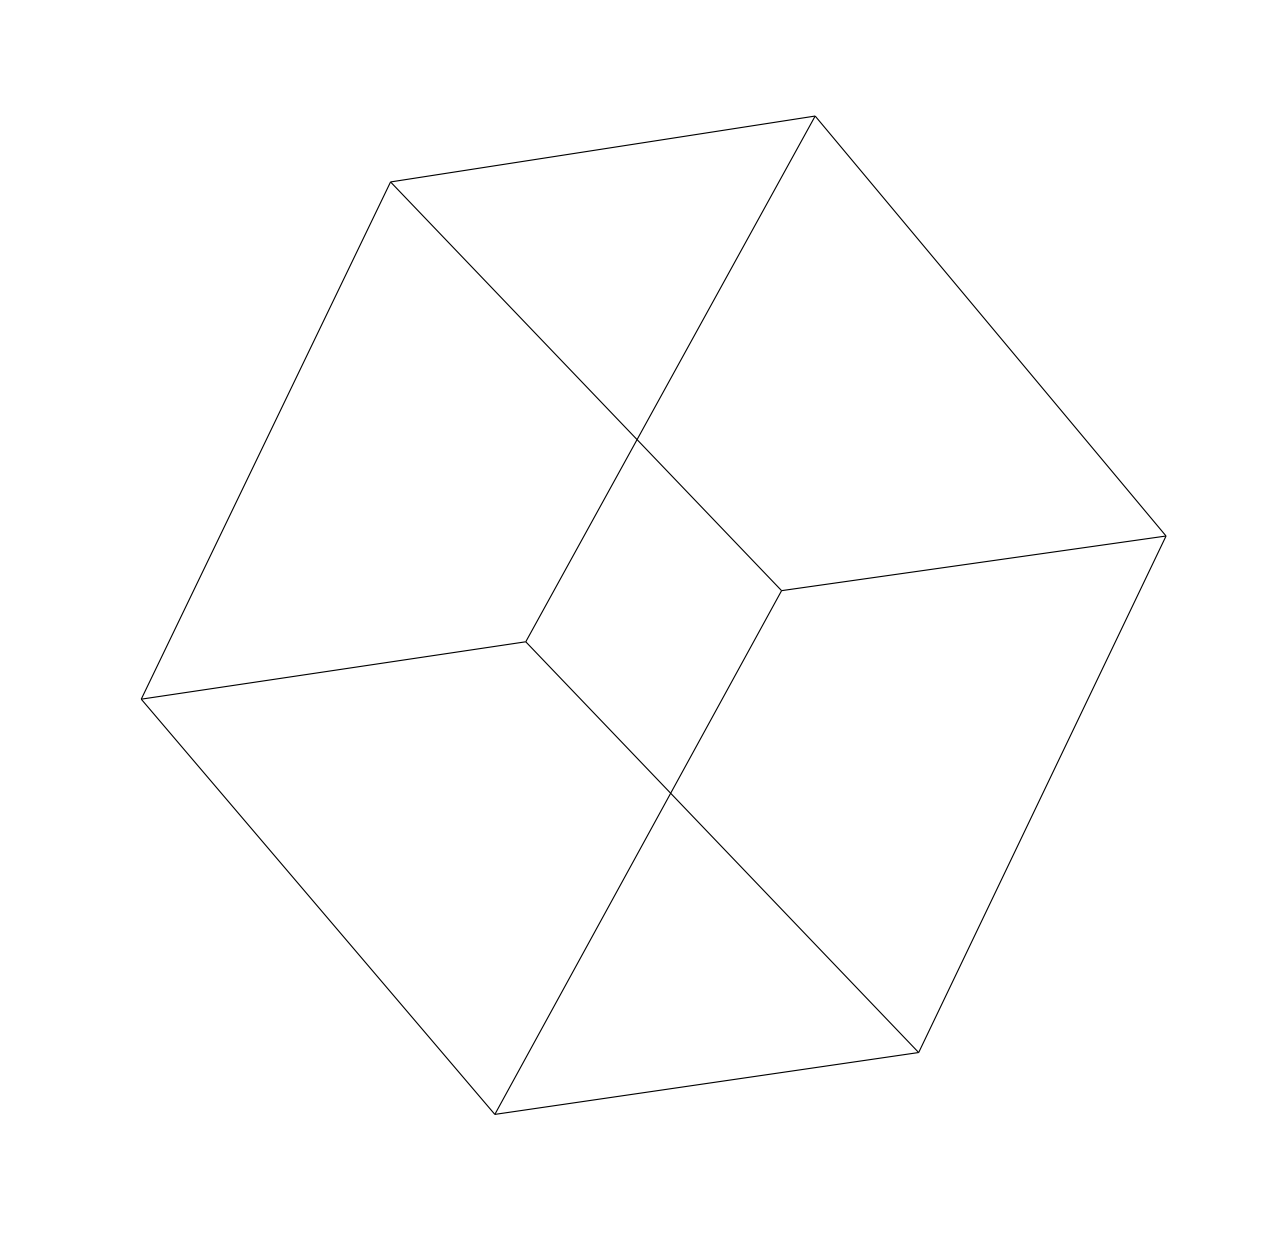
\includegraphics[width=2.2in]{./images02/new-images/qn3.png}}
  \subfloat[$Q_7$]{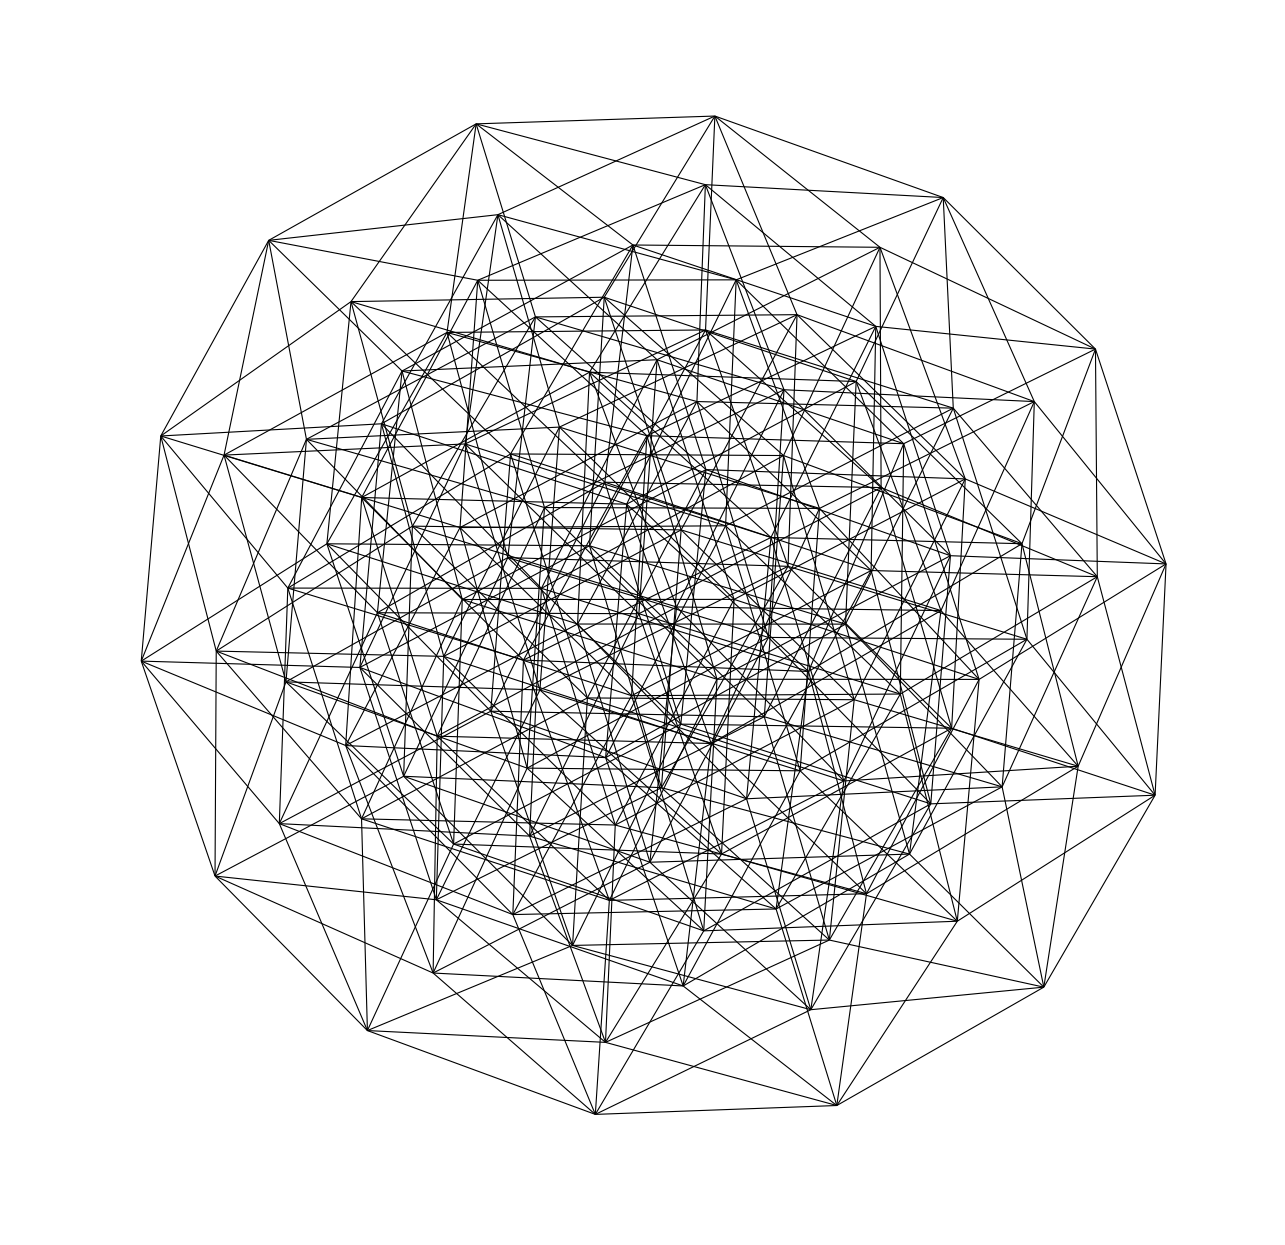
\includegraphics[width=2.2in]{./images02/new-images/qn7.png}}

  \subfloat[$Q_{10}$]{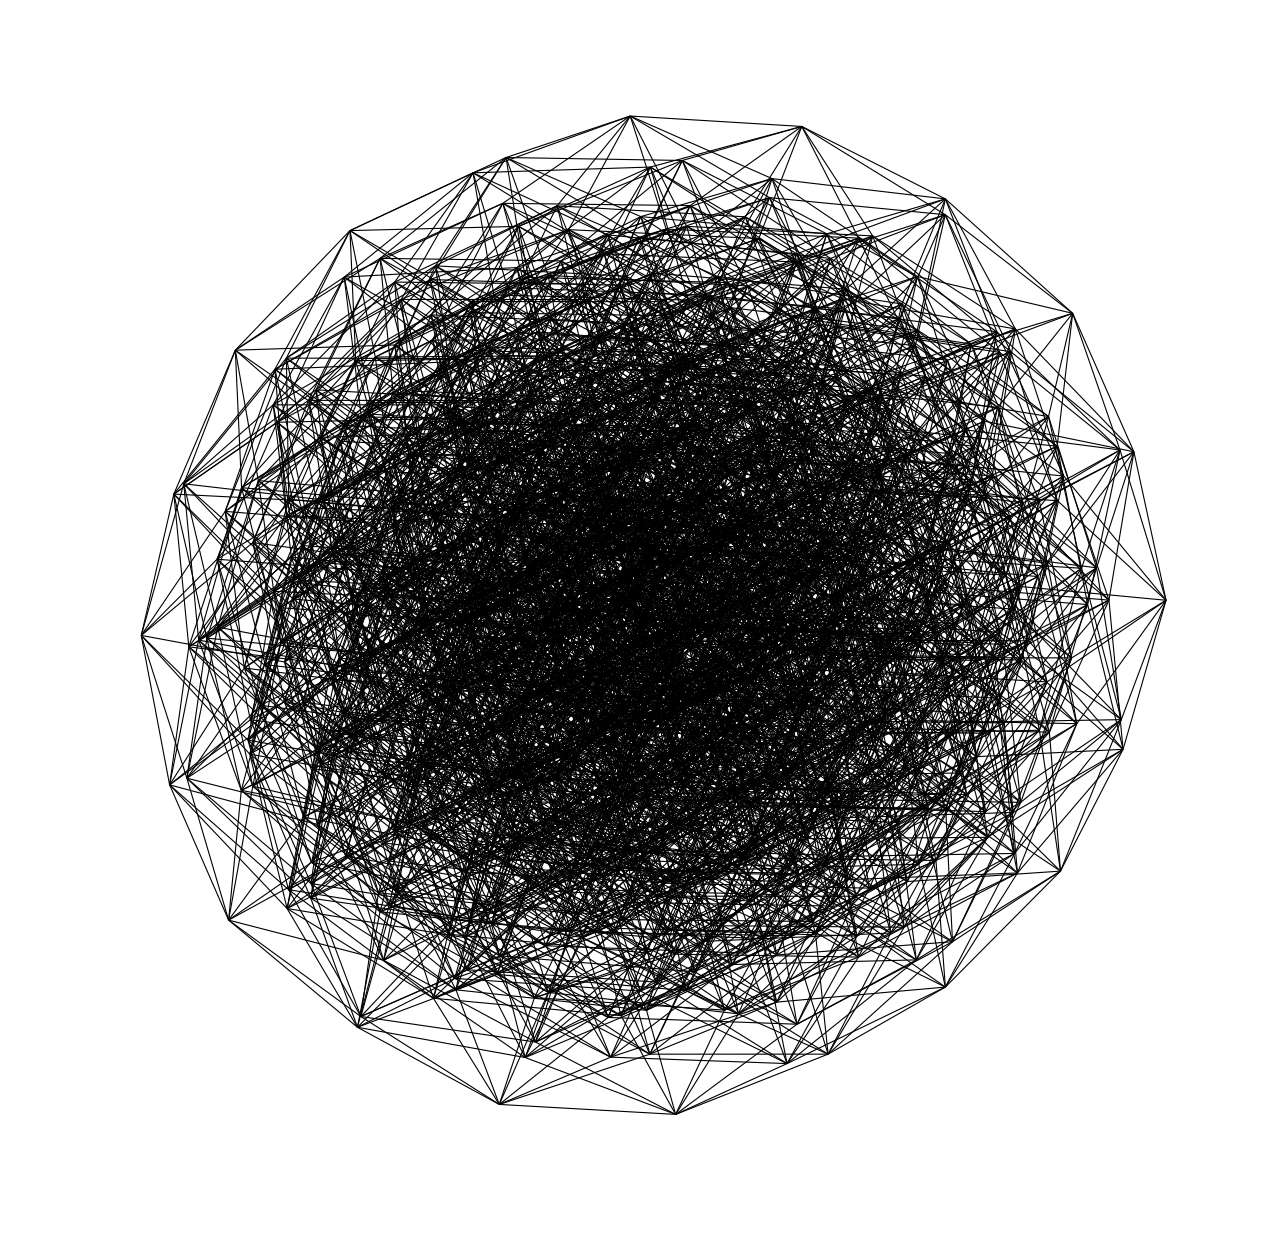
\includegraphics[width=4.0in]{./images02/new-images/qn10.png}}
  \caption{Here we have $Q_n$, for $n \in$ \{3, 7, 10\}. Each node corresponds to a bitstring in $\{0,1\}^n$, and two nodes are linked iff the bitstrings differ by a single dimension.  A number of observations can be made here. First, the number of nodes grows as $O(2^n)$; which makes the space rapidly intractable. Another interesting observation, better seen in the figures below, is that most of the space lies `at the center', at a distance of around $n/2$ from any given vantage point.\label{hypercubes}}
\end{figure}

The space studied by Kanerva is also called the \emph{hypercube graph}, or $Q_n$, as in Figure \ref{hypercubes}. For a fixed $n \in \mathbb{Z}$, the graph $G = (V, E)$, in which $v \in V$ iff there is a bijective function $b: V\to \{0,1\}^n$ and $(v_i, v_j) \in E$ iff $H(b(v_i), b(v_j))=1$, where $H$ is the Hamming distance. That is, $n$-sized bitstrings correspond to nodes, and edges exist between nodes $iff$ they flip a single bit.  Though Kanerva has derived many combinatorial properties of the space, additional results have been found by the graph-theoretical community. A good survey is provided by \citet{harary1988survey}.

One has to be careful when thinking intuitively about distance in SDM because the Hamming distance does not have the same properties of, say, our 3-dimensional space.

Though both follow the triangle inequality ($d(A, C) \le d(A, B) + d(B, C)$), which in 3-d Euclidean distance may be loosely interpreted as ``if A is close to B, and B is close to C, then A is also close to C'' --- $d(A, B) \le r \text{ and } d(B, C) \le r \Rightarrow d(A, C) \le 2r$ ---, but in SDM, although the inequality is also valid, two bitstrings would be close when, for instance, $r = 430$, so $2r = 860$ would cover all other bitstrings. Hence, it makes no sense to say that $A$ is also close to $C$.

There are numerous, beautiful, counter-intuitive notions involved in this space. This difference in intuition may trick even experienced researchers when analyzing some situations.



















Unlike traditional memory used by computers, SDM performs read and write operations in a multitude of addresses, also called neurons.  That is, the data is not written, or it is not read in a single address spot, but in many addresses. These are called activated addresses, or activated neurons.

The activation of addresses takes place according to their distances from the datum. Suppose one is writing datum $\eta$ at address $\xi$, then all addresses inside a circle with center $\xi$ and radius $r$ are activated. So, $\eta$ will be stored in all these activated addresses, which are around address $\xi$, such as in Figure \ref{fig-addresses-inside-access-radius}.  An address $\xi'$ is inside the circle if its Hamming distance to the center $\xi$ is less than or equal to the radius $r$, i.e. $distance(\xi,\xi')\leq r$.

\begin{figure}[!htb]
\centering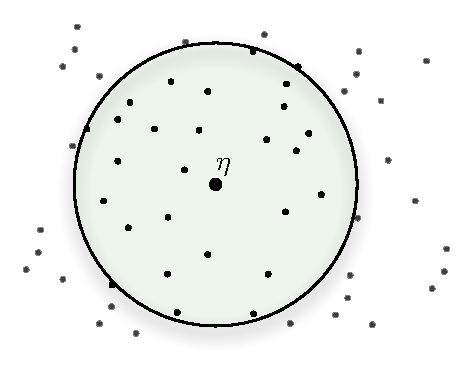
\includegraphics[scale=0.75]{./images02/p_circle_r.pdf}

\caption{Activated addresses inside access \protect \\
radius $r$ around the center address.\label{fig-addresses-inside-access-radius}}
\end{figure}



Every write or read in SDM memory activates a number of addresses with close distance.  The data is written in these activated addresses or read from them.  These issues will be addressed in due detail further on, but a major difference from a traditional computer memory is that the data are always stored and retrieved in a multitude of addresses. This way SDM memory has robustness against loss of addresses (e.g., death of a neuron).

In traditional memory, each datum is stored in an address and every lookup of a specific datum requires a search through the memory. In spite of computer scientists having developed beautiful algorithms to perform fast searches, almost all of them do a precise search. That is, if you have an imprecise clue of what you need, these algorithms will simply fail.

In SDM, the data space is the same as the address space, which amounts to a vectorial, binary space, that is, a $\{0,1\}^{n}$ space. This way, the addresses where the data will be written are the same as the data themselves. For example, the datum $\eta=00101_{b}\in\{0,1\}^{5}$ will be written to the address $\xi=\eta=00101_{b}$. If one chooses a radius of 1, the SDM will activate all addresses one bit away or less from the center address. So, the datum $00101_{b}$ will be written to the addresses $00101_{b}$, $10101_{b}$, $01101_{b}$, $00001_{b}$, $00111_{b}$, and $00100_{b}$.

In this case, when one needs to retrieve the data, one could have an imprecise cue at most one bit away from $\eta$, since all addresses one bit away have $\eta$ stored in themselves.  Extending this train of thought for larger dimensions and radius, exponential numbers of addresses are activated and one can see why SDM is a distributed memory.

When reading a cue $\eta_{x}$ that is $x$ bits away from $\eta$, the cue shares many addresses with $\eta$. The number of shared addresses decreases as the cue's distance to $\eta$ increases, in other words, as $x$ increases. This is shown in Figure \ref{fig-shared-addresses}.  The target datum $\eta$ was written in all shared addresses, thus they will bias the read output in the direction of $\eta$. If the cue is sufficiently near the target datum $\eta$, the read output will be closer to $\eta$ than $\eta_{x}$ was. Repeating the read operation increasingly gets results closer to $\eta$, until it is precisely the same. So, it may be necessary to perform more than one read operation to converge to the target data $\eta$.

\begin{figure}[!htb]
\centering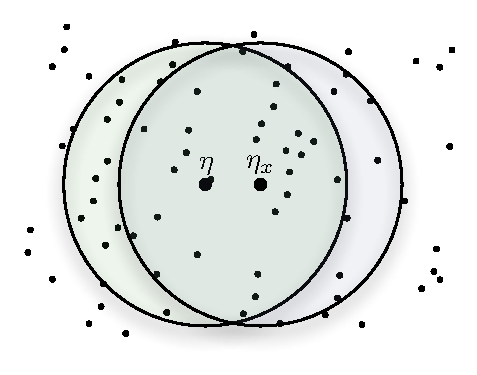
\includegraphics[scale=0.75]{./images02/p1_inter_p2.pdf}

\caption{Shared addresses between the \protect \\
target datum $\eta$ and the cue $\eta_{x}$. \label{fig-shared-addresses}}
\end{figure}


The addresses of the $\{0,1\}^{n}$ space grow exponentially with the number of dimensions $n$, i.e., $N=2^{n}$. For $n=100$ we have $N\approx10^{30}$, which is incredibly large when related to computer memory. Furthermore, \citet{Kanerva1988} suggests $n$ between 100 and 10,000. Recently he has postulated 10,000 as a desirable minimum $N$ (personal communication). To solve the feasibility problem of implementing this memory, Kanerva made a random sample of $\{0,1\}^{n}$, in his work, having $N'$ elements. All these addresses in the sample are called hard locations. Other elements of $\{0,1\}^{n}$, not in $N'$, are called virtual neurons. This is represented in Figure \ref{fig-hardlocations}.  All properties of reading and write operations presented before remain valid but limited to hard locations. Kanerva suggests taking a sample of about one million hard locations.

Using this sample of binary space, our data space does not exist completely.  That is, the binary space has $2^{n}$ addresses, but the memory is far away from having these addresses available. In fact, only a fraction of this vectorial space is actually instantiated. Following Kanerva's suggestion of one million hard locations, for $n=100$, only $100\cdot10^{6}/2^{100}=7\cdot10^{-23}$ percent of the whole space exists, and for $n=1,000$ only $100\cdot10^{6}/2^{1000}=7\cdot10^{-294}$ percent.

Kanerva also suggests the selection of a radius that will activate, on average, one-thousandth of the sample, which is 1,000 hard locations for a sample of one million addresses. In order to achieve his suggestion, a 1,000-dimension memory uses an access radius $r=451$, and a 256-dimensional memory, $r=103$. We think that a 256-dimensional memory may be important because it presents conformity to Miller's magic number \citep{Linhares2011}.

\begin{figure}[!htb]
\centering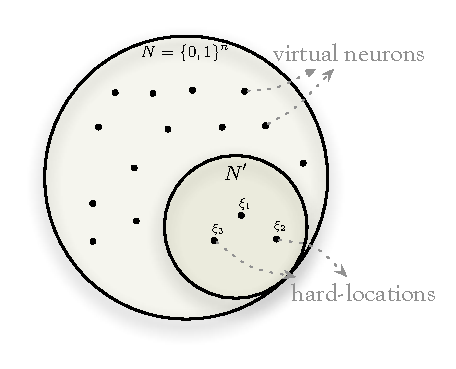
\includegraphics[scale=0.75]{./images02/hardlocations.pdf}

\caption{Hard-locations randomly sampled from binary space.\label{fig-hardlocations}}
\end{figure}


Since a cue $\eta_{x}$ near the target bitstring $\eta$ shares many hard locations with $\eta$, SDM can retrieve data from imprecise cues. Despite this feature, it is very important to know how imprecise this cue could be while still giving accurate results. What is the maximum distance from our cue to the original data that still retrieves the right answer? An interesting approach is to perform a read operation with a cue $\eta_{x}$, that is $x$ bits away from the target $\eta$.  Then measure the distance from the read output and $\eta$. If this distance is smaller than $x$ we are converging. Convergence is simple to handle, just read again and again, until it converges to the target $\eta$. If this distance is greater than $x$ we are diverging. Finally, if this distance equals $x$ we are in a tip-of-the-tongue process.  A tip-of-the-tongue psychologically happens when you know that you know, but you can't say what exactly it is. In SDM mathematical model, a tip-of-the-tongue process takes infinite time to converge. \citet{Kanerva1988} called this $x$ distance, where the read's output averages $x$, the critical distance. Intuitively, it is the distance from which smaller distances converge and greater distances diverge. In Figure \ref{fig-p1-p2-iterative-read}, the circle has radius equal to the critical distance and every $\eta_{x}$ inside the circle should converge.  The figure also shows convergence in four readings.

\begin{figure}[!htb]
\centering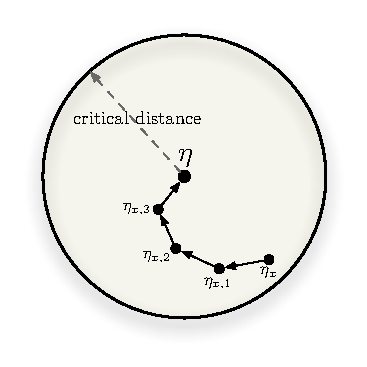
\includegraphics[scale=0.75]{./images02/p1_p2_iter_read.pdf}

\caption{In this example, four iterative readings were\protect \\
required to converge from $\eta_{x}$ to $\eta$.\label{fig-p1-p2-iterative-read}}
\end{figure}


The $\{0,1\}^{n}$ space has $N=2^{n}$ locations from which we instantiate $N'$ samples. Each location in our sample is called a hard location.  On these hard locations, we do operations of read and write. One of the insights of SDM is exactly the way we read and write: using data as addresses in a distributed fashion. Each datum $\eta$ is written in every activated hard location inside the access radius centered on the address, that equals datum, $\xi=\eta$. Kanerva suggested using an access radius $r$ having about one-thousandth of $N'$.  As an imprecise cue $\eta_{x}$ shares hard locations with the target bitstring $\eta,$ it is possible to retrieve $\eta$ correctly. (Actually, probably more than one read is necessary to retrieve exactly $\eta.)$.  Moreover, if some neurons are lost, only a fraction of the datum is lost and it is possible that the memory can still retrieve the right datum.

A random bitstring is generated with equal probability of $0$'s and $1$'s for each bit. One can readily see that the average distance between two random bitstrings follows the binomial distribution with mean $n/2$ and standard deviation $\sqrt{n/4}$. For a large $n$, most of the space lies close to the mean and has fewer shared hard locations.  As two bitstrings with distance far from $n/2$ are very improbable, \citet{Kanerva1988} defined that two bitstrings are orthogonal when their distance is $n/2$.

The write operation needs to store, for each dimension bit which happened more ($0$'s or $1$'s). This way, each hard location has $n$ counters, one for each dimension. The counter is incremented for each bit $1$ and decremented for each bit $0$. Thus, if the counter is positive, there have been more $1$'s than $0$'s, if the counter is negative, there have been more $0$'s than $1$'s, and if the counter is zero, there have been an equal number of $1$'s and $0$'s. Table \ref{tab:write operation} shows an example of a write operation being performed in a 7-dimensional memory.

\begin{table}
\begin{tabular}{c|c|c|c|c|c|c|c|}
\cline{2-8}
$\eta$ & 0 & 1 & 1 & 0 & 1 & 0 & 0\tabularnewline
\cline{2-8}
$\xi_{\textit{before}}$ & 6 & -3 & 12 & -1 & 0 & 2 & 4\tabularnewline
\cline{2-8}
\multicolumn{1}{c}{} & \multicolumn{1}{c}{\textcolor{red}{\small{}$\Downarrow$ -1}} & \multicolumn{1}{c}{\textcolor{red}{\small{}$\Downarrow$ +1}} & \multicolumn{1}{c}{\textcolor{red}{\small{}$\Downarrow$ +1}} & \multicolumn{1}{c}{\textcolor{red}{\small{}$\Downarrow$ -1}} & \multicolumn{1}{c}{\textcolor{red}{\small{}$\Downarrow$ +1}} & \multicolumn{1}{c}{\textcolor{red}{\small{}$\Downarrow$ -1}} & \multicolumn{1}{c}{\textcolor{red}{\small{}$\Downarrow$ -1}}\tabularnewline
\cline{2-8}
$\xi_{\textit{\textit{after}}}$ & \textbf{5} & \textbf{-2} & \textbf{13} & \textbf{-2} & \textbf{1} & \textbf{1} & \textbf{3}\tabularnewline
\cline{2-8}
\end{tabular}

\caption{Write operation example in a 7-dimensional memory of data $\eta$
being written to $\xi$, one of the activated addresses.\label{tab:write operation}}


\end{table}


The read is performed polling each activated hard location and statistically choosing the most written bit for each dimension. It consists of adding all $n$ counters from the activated hard locations and, for each bit, choosing bit 1 if the counter is positive, choosing bit 0 if the counter is negative, and randomly choose bit 0 or 1 if the counter is zero.


\section{Neurons as pointers}

One interesting view is that neurons in SDM work like pointers. As we write bitstrings in memory, the hard locations' counters are updated and some bits are flipped. Thus, the activated hard locations do not necessarily point individually to the bitstring that activated it, but together they point correctly. In other words, the read operation depends on many hard locations to be successful. This effect is represented in Figure \ref{fig-p1-pointers}: where all hard locations inside the circle are activated and they, individually, do not point to $\eta$.  But, like vectors, adding them up points to $\eta$. If another datum $\nu$ is written into the memory near $\eta$, the shared hard locations will have information from both of them and would not point to either.  All hard locations outside of the circle are also pointing somewhere (possibly other data points). This is not shown, however, in order to keep the picture clean and easily understandable.

\begin{figure}[!htb]
\centering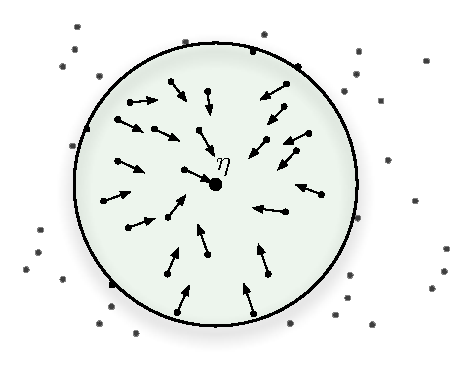
\includegraphics[scale=0.75]{./images02/p1_after_write.pdf}

\caption{Hard-locations pointing, approximately, to the target bitstring.\label{fig-p1-pointers}}
\end{figure}



\section{Concepts}

Although Kanerva does not mention concepts directly in his book \citep{Kanerva1988}, the author's interpretation is that each bitstring may be mapped to a concept. Thus, unrelated concepts are orthogonal and concepts could be linked through a bitstring near both of them. For example, ``beauty'' and ``woman'' have distance $n/2$, but a bitstring that means ``beautiful woman'' could have distance $n/4$ to both of them. As a bitstring with distance $n/4$ is very improbable, it is linking those concepts together. \citet{Linhares2011} approached this concept via ``chunking through averaging''.

Due to the distribution of hard locations between two random bitstrings, the vast majority of concepts is orthogonal to all others. Consider a non-scientific survey during a cognitive science seminar, where students asked to mention ideas unrelated to the course brought up terms like birthdays, boots, dinosaurs, fever, executive order, x-rays, and so on. Not only are the items unrelated to cognitive science, the topic of the seminar, but they are also unrelated to each other.

For any two memory items, one can readily find a stream of thought relating two such items (``Darwin gave dinosaurs the boot''; ``she ran a fever on her birthday''; ``isn't it time for the Supreme Court to x-ray that executive order?'', ... and so forth). Robert French presents an intriguing example in which one suddenly creates a representation linking the otherwise unrelated concepts of ``coffee cups'' and ``old elephants'' \citep{French1997}.

This mapping from concepts to bitstrings brings us two central questions: (i) Suppose we have a bitstring that is linking two major concepts.  How do we know which concepts are linked together? (ii) From a concept bitstring, how can we list all concepts that are somehow linked to it? This second question is called the problem of spreading activation.


\section{Read operation}

In his work, Kanerva proposed and analyzed a read algorithm called here Kanerva's read. His read takes all activated hard locations counters and sum them. The resulting bitstring has bit $1$ where the result is positive, bit $0$ where the result is negative, and a random bit where the result is zero. In a word, each bit is chosen according to all written bitstrings in all hard locations, being equal to the bit more appeared. Table \ref{tab:kanerva-read} shows an example of Kanerva's read result bitstring.

Daniel Chada, one member of our research group, proposed another way to read in SDM, in this work called Chada's read. Instead of summing all hard location counters, each hard location evaluates its resulting bitstring individually. Then, all resulting bitstrings are summed again, and the same rule as Kanerva applies. Table \ref{tab:chada-read} shows an example of Chada's read result bitstring. The counter's values are normalized to 1, for positive ones, or -1, for negative ones, and the original values are the same as in Table \ref{tab:kanerva-read}.

The main difference between Kanerva's read and Chada's is that, in the former, a hard location that has more bitstrings written has a greater weight in the decision of each bit. In the latter, all hard locations have the same weight, because they can contribute to the sum with only one bitstring.

It is important to say that Chada's read came from \citet{anwar2003sparse} which gave a misguided description of the read operation. The original description is the following:

\begin{samepage}
\begin{quote}
%Similar to writing, retrieving from SDM involves the same concept of access sphere --- you read all the hardlocations within the access sphere of location Y, pool the bit vectors read from all these hard locations and let each of the kth bits of those locations participate in a majority vote for the kth bit of Y. \hfill --- \citet{anwar2003sparse}
With our datum distributively stored, the next question is how to retrieve it. With this in mind, let us ask first how one reads from a single hard location, $x$. Compute $\zeta$, the bit vector read at $x$, by assigning its $i$th bit the value 1 or 0 according to the $i$th counter at $x$ is positive or negative. Thus, each bit of $\zeta$ results from a majority rule decision of all the data that have been written at $x$. [...] Knowing how to read from a hard location allows us to read from any of the $2^{1000}$ arbitrary locations. Suppose $\zeta$ is any location. The bit vector, $\xi$, to be read at $\zeta$, [...] Put another way, pool the bit vectors read from hard locations accessible from $\zeta$, and let each of their $i$th bits vote on the $i$th bit of $\xi$. \\
\hfill --- \citet[p.342]{anwar2003sparse}
\end{quote}
\end{samepage}

This fact just highlights how important it is to have a reference implementation that one may read the code to clarify one's understanding about the details of each operation.

\subsection{Generalized read operation}

A member of my Master's committee, Prof. Paulo Murilo\footnote{Universidade Federal Fluminense's Physics Professor Paulo Murilo}, has proposed a generalized reading operation (personal communication), which covers both Kanerva's and Chada's read --- and opens a new venue of potential discoveries. He proposed summing all hard location counters raised to the power of $z$ while holding the original sign of the counter (positive or negative). Thus, Kanerva's read would be the same as $z=1$, while Chada's would be the same as $z=0$. Hence, we will here explore how SDM would behave with other values of $z$, such as 0.5, 2, and 3. Mathematically, let $A$ be the set of the counters of the activated hard location, and $c_i$ be the counter of the $i$th bit. Then,

$$
s_i = \sum_{c \in A} \frac{c_i}{|c_i|} |c_i|^z
$$

Finally, the $i$th bit of the resulting bitstring is 1 if $s_i > 0$, or 0 if $s_i < 0$, or random if $s_i = 0$. Notice that when $z=1$, then $s_i = \sum_{c \in A} c_i$, which is the Kanerva's read; and when $z=0$, then $s_i = \frac{c_i}{|c_i|} = \text{sign}(c_i)$, which is the Chada's read.

\begin{table}
\begin{minipage}[t]{0.5\columnwidth}%
\subfloat[Kanerva's read example\label{tab:kanerva-read}]{%
\begin{tabular}{c|c|c|c|c|c|}
\cline{2-6}
$\xi_{1}$ & -2 & 12 & 4 & 0 & -3\tabularnewline
\cline{2-6}
$\xi_{2}$ & -5 & -4 & 2 & 8 & -2\tabularnewline
\cline{2-6}
$\xi_{3}$ & -1 & 0 & -1 & -2 & -1\tabularnewline
\cline{2-6}
$\xi_{4}$ & 3 & 2 & -1 & 3 & 1\tabularnewline
\hline
\multicolumn{1}{|c|}{\textbf{$\sum$}} & \textbf{-5} & \textbf{10} & \textbf{4} & \textbf{3} & \textbf{-5}\tabularnewline
\hline
\multicolumn{1}{c}{} & \multicolumn{1}{c}{\textcolor{red}{\small{}$\Downarrow$}} & \multicolumn{1}{c}{\textcolor{red}{\small{}$\Downarrow$}} & \multicolumn{1}{c}{\textcolor{red}{\small{}$\Downarrow$}} & \multicolumn{1}{c}{\textcolor{red}{\small{}$\Downarrow$}} & \multicolumn{1}{c}{\textcolor{red}{\small{}$\Downarrow$}}\tabularnewline
\cline{2-6}
 & 0 & 1 & 1 & 1 & 0\tabularnewline
\cline{2-6}
\end{tabular}

}%
\end{minipage}%
\begin{minipage}[t]{0.5\columnwidth}%
\subfloat[Chada's read example\label{tab:chada-read}]{%
\begin{tabular}{c|c|c|c|c|c|}
\cline{2-6}
$\xi_{1}$ & -1 & 1 & 1 & \cellcolor{lightgray}1 & -3\tabularnewline
\cline{2-6}
$\xi_{2}$ & -1 & -1 & 1 & 1 & -1\tabularnewline
\cline{2-6}
$\xi_{3}$ & -1 & \cellcolor{lightgray}1 & -1 & -1 & -1\tabularnewline
\cline{2-6}
$\xi_{4}$ & 1 & 1 & -1 & -1 & 1\tabularnewline
\hline
\multicolumn{1}{|c|}{\textbf{$\sum$}} & \textbf{-2} & \textbf{1} & \textbf{0} & \textbf{0} & \textbf{-2}\tabularnewline
\hline
\multicolumn{1}{c}{} & \multicolumn{1}{c}{\textcolor{red}{\small{}$\Downarrow$}} & \multicolumn{1}{c}{\textcolor{red}{\small{}$\Downarrow$}} & \multicolumn{1}{c}{\textcolor{red}{\small{}$\Downarrow$}} & \multicolumn{1}{c}{\textcolor{red}{\small{}$\Downarrow$}} & \multicolumn{1}{c}{\textcolor{red}{\small{}$\Downarrow$}}\tabularnewline
\cline{2-6}
 & 0 & 1 & \cellcolor{lightgray}1 & \cellcolor{lightgray}1 & 0\tabularnewline
\cline{2-6}
\end{tabular}

}%
\end{minipage}\caption{Comparison of Kanerva's read and Chada's read. Each $\xi_{i}$ is
an activated hard location and the values come from their counters.
Gray cells' value is obtained randomly with probability 50\%.\label{tab:read-operation}}
\end{table}


\section{Critical Distance}

Kanerva describes the critical distance as the threshold of convergence of a sequence of read words. It is ``the distance beyond which divergence is more likely than convergence''\citep{Kanerva1988}. Furthermore, Kanerva explains that ``a very good estimate of the critical distance can be obtained by finding the distance at which the arithmetic mean of the new distance to the target equals the old distance to the target''\citep{Kanerva1988}.  In other words, the critical distance can be equated as the edge to our memory, the limit of human recollection.

In his book, Kanerva analyzed a specific situation with $n=1000$ ($N=2^{1000}$), 1 million hard locations ($N'=1,000,000$), an access-radius of 451 (within 1,000 hard locations in each circle), and 10 thousand writes of random bitstrings in the memory. As computer resources were very poor those days, Kanerva couldn't make a more generic analysis.

Starting from the premise of SDM as a faithful model of human short-term memory, a better understanding of the critical distance may shed light on our understanding of the thresholds that bind our own memory.


\begin{figure}[!htb]
\centering

\subfloat[Kanerva's original model]{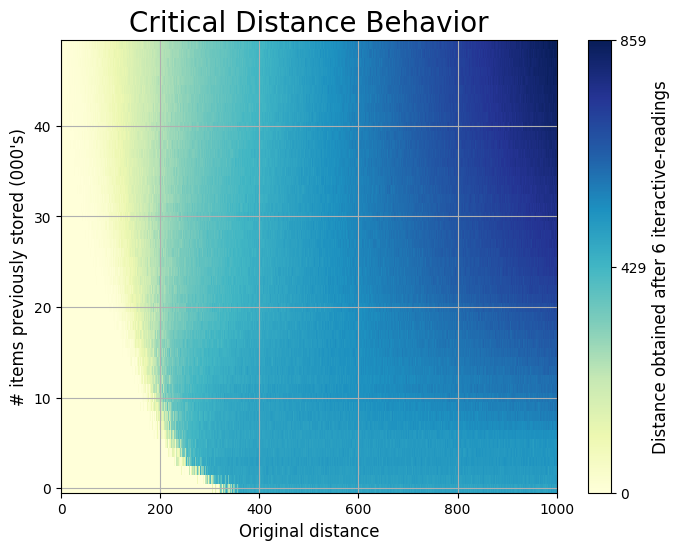
\includegraphics[width=3.1in]{./images02/new-images/kanerva-read.png}\label{fig:cir-dist-10k-writes-kanerva}}

\subfloat[Chada's read]{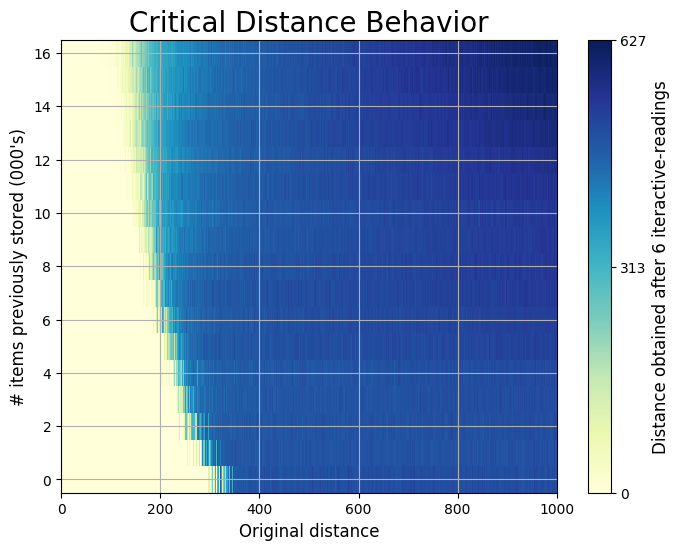
\includegraphics[width=3.1in]{./images02/new-images/chada-read_z_0.png}}
\caption{How far, in Hamming distance, is a read item from the original stored item? Kanerva demonstrated that, after a small number of iterative readings (6 here), a critical distance behavior emerges. Items read at close distance converge rapidly; whereas farther items do not converge. Most striking is the point in which the system displays the tip-of-tongue behavior. Described by psychological moments when some features of the item are prominent in one's thoughts, yet the item still cannot be recalled (but an additional cue makes convergence `immediate'). Mathematically, this is the precise distance in which, despite having a relatively high number of cues (correct bits) about the desired item, the time to convergence is infinite.   Heatmap colors display the Hamming distance the associative memory is able to cleanly converge to---or not.   In the $x$-axis, the distance from the desired item is displayed. In the $y$-axis, we display the read operation's behavior as the number of items registered in the memory grows.  These graphs are computing intensive, yet they can be easily tested by readers in our provided Jupyter notebooks. Note the different scales.}
\label{fig:crit-dist-10k-writes}

\end{figure}

Figure \ref{fig:crit-dist-10k-writes} compares the critical distance behavior under different scenarios.  This replicates our previous results \citep{Brogliato2011, brogliato2014sparse} and is a first part of the process of framework validation, to which we throw our attention next.
